\let\negmedspace\undefined
\let\negthickspace\undefined
\documentclass[journal]{IEEEtran}
\usepackage[a5paper, margin=10mm, onecolumn]{geometry}
\usepackage{lmodern} % Ensure lmodern is loaded for pdflatex
\usepackage{tfrupee} % Include tfrupee package

\setlength{\headheight}{1cm} % Set the height of the header box
\setlength{\headsep}{0mm}     % Set the distance between the header box and the top of the text

\usepackage{gvv-book}
\usepackage{gvv}
\usepackage{cite}
\usepackage{amsmath,amssymb,amsfonts,amsthm}
\usepackage{algorithmic}
\usepackage{graphicx}
\usepackage{textcomp}
\usepackage{xcolor}
\usepackage{txfonts}
\usepackage{listings}
\usepackage{enumitem}
\usepackage{mathtools}
\usepackage{gensymb}
\usepackage{comment}
\usepackage[breaklinks=true]{hyperref}
\usepackage{tkz-euclide} 
\usepackage{listings}
 \usepackage{gvv}                                        
\def\inputGnumericTable{}                                 
\usepackage[latin1]{inputenc}                                
\usepackage{color}                                            
\usepackage{array}                                            
\usepackage{longtable}                                       
\usepackage{calc}                                             
\usepackage{multirow}                                         
\usepackage{hhline}                                           
\usepackage{ifthen}                                           
\usepackage{lscape}
\begin{document}

\bibliographystyle{IEEEtran}


\title{1.5.9}
\author{EE25BTECH11021 - Dhanush Sagar
}
% \maketitle
% \newpage
% \bigskip
{\let\newpage\relax\maketitle}

\renewcommand{\thefigure}{\theenumi}
\renewcommand{\thetable}{\theenumi}
\setlength{\intextsep}{10pt} % Space between text and floats


\numberwithin{equation}{enumi}
\numberwithin{figure}{enumi}
\renewcommand{\thetable}{\theenumi}



\textbf{Problem (1.5.9).} Find the ratio in which the Y-axis divides the line segment joining
\begin{align}
    A=\myvec{5\\-6} \quad \text{and} \quad B=\myvec{-1\\-4}.
\end{align}
Also, find the coordinates of the point of intersection.

\textbf{Solution:}\\
 given points are A and B
\begin{align*} \vec{A} = \myvec{5 \\ -6}, \vec{B} = \myvec{-1 \\ -4} \end{align*}
Let the Y-axis divide the \(\overline{\vec{AB}}\) at point $\vec{P}$ in the ratio $k:1$.
Since $\vec{P}$ lies on Y-axis, let intersection point P be
\begin{align*}
\vec{P} = \myvec{0 \\ y}
\end{align*}
The point $\vec{A}$, $\vec{B}$, $\vec{P}$ are collinear.
\begin{align}
\implies \text{rank}\myvec{\vec{B}-\vec{A} & \vec{P}-\vec{A}} = 1
\end{align}
\begin{align}
\myvec{-6 & -5 \\ 2 & y+6} \xleftrightarrow[]{R_2 \rightarrow {\frac{1}{3}R_1 + R_2}}\myvec{-6 & -5 \\ 0 & y+\frac{13}{3}}  
\end{align}
The number of nonzero rows in the row reduced matrix is defined as the rank. For above matrix to be of rank 1,
\begin{align}
y+\frac{13}{3} &= 0 \\
y &= \frac{-13}{3}
\end{align}
$\therefore$ The coordinates of the point of intersection are 
\begin{align*}
\vec{P} = \myvec{0 \\ \frac{-13}{3}}
\end{align*}

Substituting the values of $\vec{A}$, $\vec{B}$ and $\vec{P}$,
\begin{align}
k=\frac{\myvec{5 & \frac{-5}{3}}\myvec{1 \\ \frac{-1}{3}}}{\norm{\myvec{1 \\ \frac{-1}{3}}}^2}=5
\end{align}



\begin{figure}[H]
    \centering
    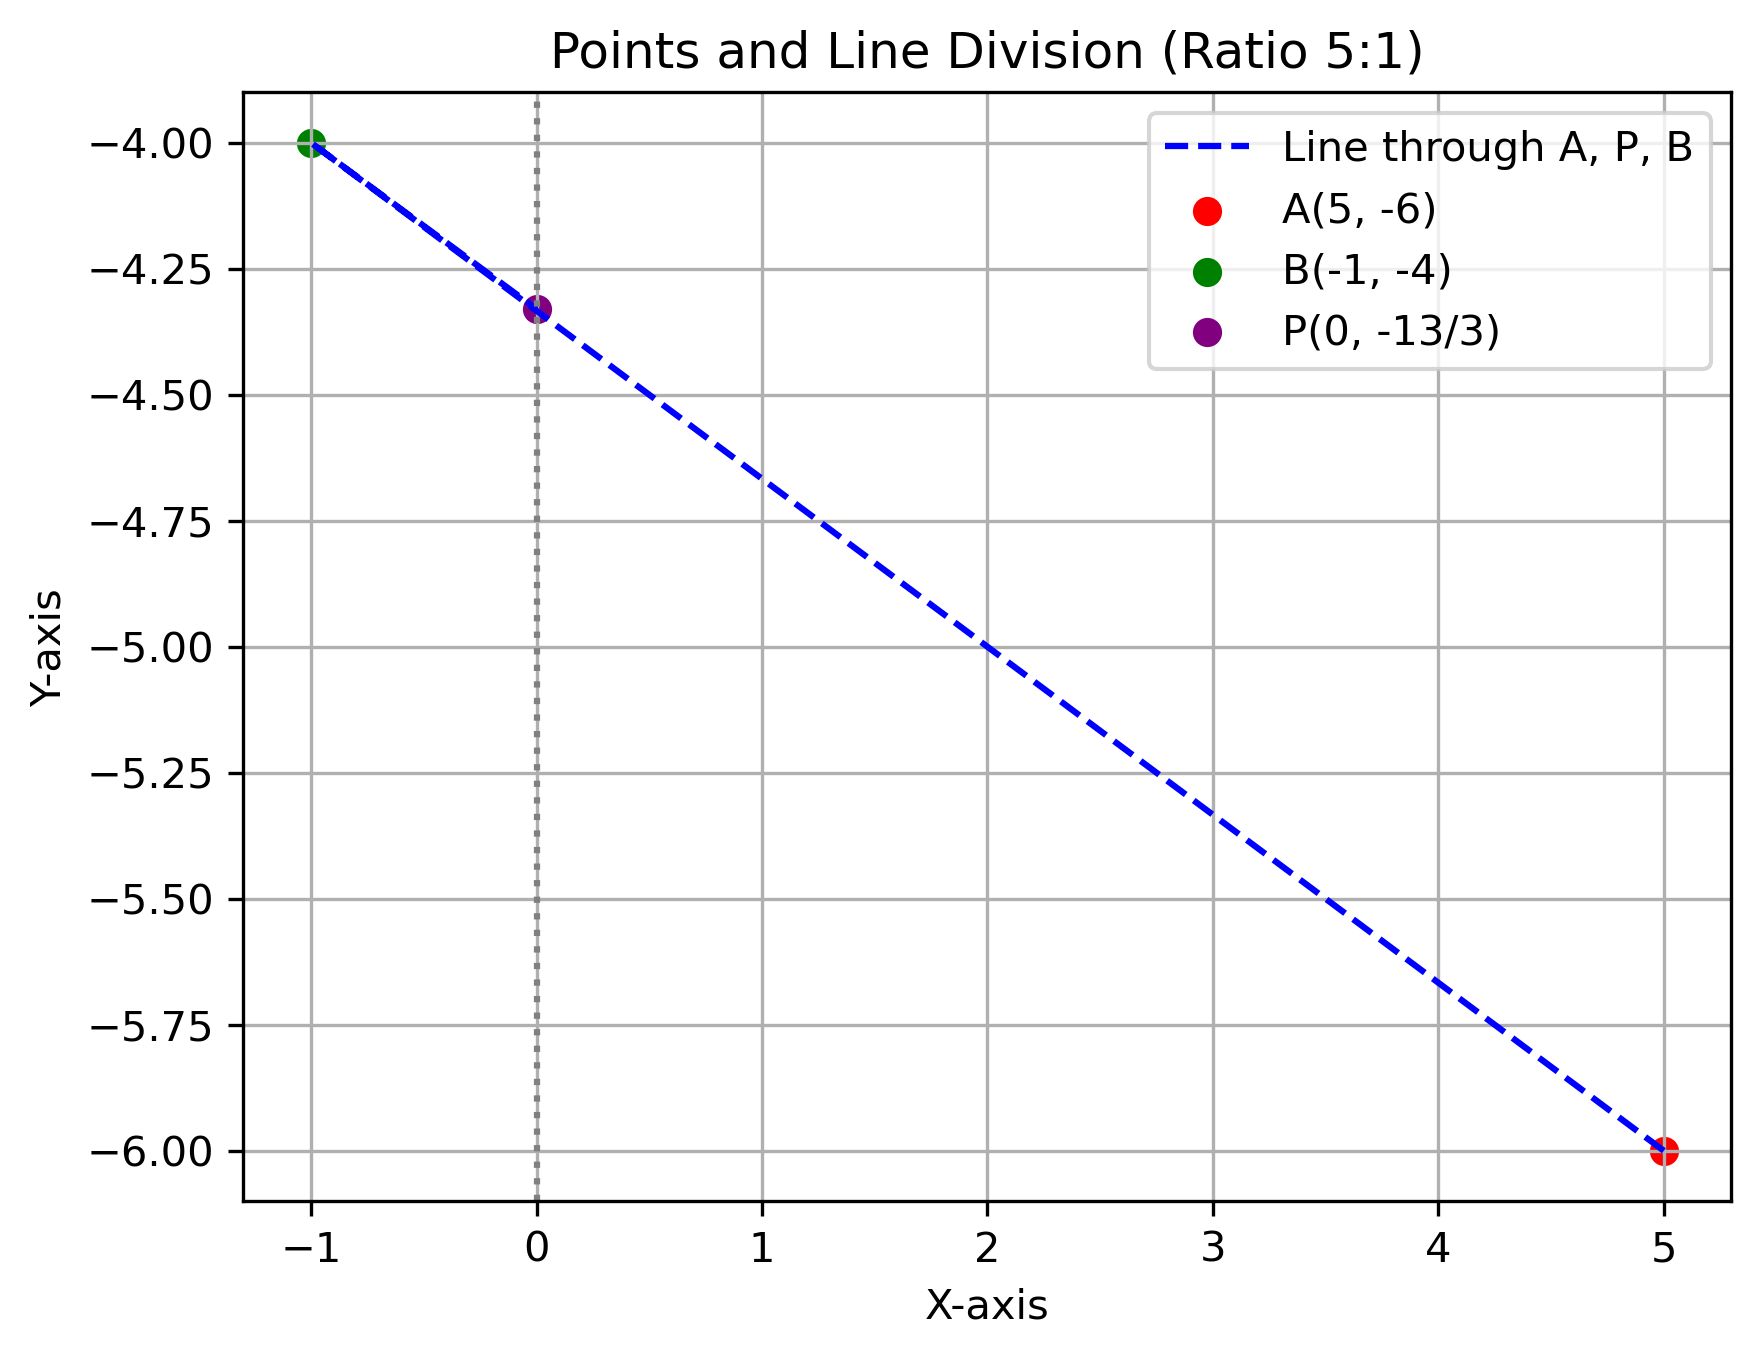
\includegraphics[width=0.5\columnwidth]{figs/fig1.png}
    \caption{}
    \label{fig:fig1}
\end{figure}



\textbf{Answer:} The Y-axis divides \(\overline{AB}\) in the ratio \(5:1\) (internally), and the intersection point is
\begin{align}
\boxed{\;P=\myvec{0\\[4pt]-\dfrac{13}{3}}\;}
\end{align}

\end{document}


